\documentclass[10pt,a4paper]{article}
\usepackage[utf8]{inputenc}
\usepackage[german]{babel}
\usepackage{amsmath}
\usepackage{amsfonts}
\usepackage{amssymb}
\usepackage{siunitx}
\usepackage[left=2cm,right=2cm,top=2cm,bottom=2cm]{geometry}
\usepackage{wrapfig}
\usepackage{graphicx}
\usepackage[outdir=./]{epstopdf}
\usepackage{caption}
\usepackage[colorlinks]{hyperref}
\usepackage{pdflscape}

\author{Christian Bespin \and Christopher Deutsch}
\title{Übungsblatt 4: Numerische Methoden der Physik}
\begin{document}
\maketitle

\setcounter{section}{1}

\section{Widerstandswürfel}

\subsection{Physikalischer Hintergrund}

Zur Berechnung des Gesamtwiderstands werden die Zusammenhänge zwischen den einzelnen, auf jeder Kante liegenden, Widerständen bestimmt. Hierzu wird die Kirchhoff'sche Maschenregel verwendet, nach der die Summe aller Spannungen in einer Masche des Netzwerks $0$ ergibt. Sie folgt unmittelbar aus dem Gauß'schen Satz:
\begin{align}
\oint_A \vec{E}\,\mathrm{d}\vec{A}=\frac{Q}{\epsilon_0}
\end{align}
Die Spannungen an den Widerständen werden mit dem Ohmschen Gesetz ($U=R I$) aus $I$ und $R$ berechnet. Es lassen sich im Fall des Würfels $6$, beim Oktaeder $8$ Maschen finden, für die je eine Gleichung aufgestellt wird, mit denen sich ein lineares Gleichungssystem in Matrixschreibweise aufstellen lässt (REFS). Wir berechnen also den Vektor mit Komponenten $I_i, I_{ges}$, um von dem Gesamtstrom mit erneuter Verwendung des Ohm'schen Gesetzes auf den Gesamtwiderstand $R_{ges}$ zu schließen.
\begin{wrapfigure}[14]{R}[1pt]{0.35\textwidth}
\centering
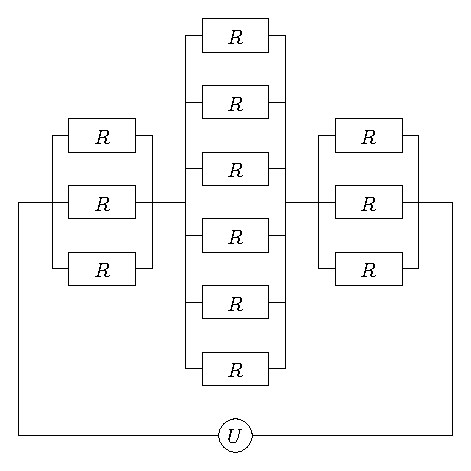
\includegraphics[width=0.3\textwidth]{./figures/ersatzschaltbild.eps}
\caption{Schaltbild für gleiche Widerstände $R$}
\label{fig:ersatzschaltbild}
\end{wrapfigure}

\noindent Für den Fall, dass alle verwendeten Widerstände gleich sind, lassen sich alle Ecken gleichen Potenzials verbinden und man erhält ein einfaches Ersatzschaltbild (Abb. \ref{fig:ersatzschaltbild}). Man nutzt nun aus, dass sich Widerstände in Parallelschaltungen reziprok und in Reihenschaltungen gewöhnlich addieren. Man erhält somit schnell:
\begin{align}
R_{ges}=\left( 3\,R\right)^{-1}+\left( 6\,R\right)^{-1}+\left( 3\,R\right)^{-1}=\frac{5}{6}\,R
\end{align}




\subsubsection{Oktaeder}

\subsection{Implementierung}

\subsubsection{Nullstellenberechnung mit Bisektion}

\subsubsection{Numerische Integration mit rekursivem Simpson-Verfahren}


\subsubsection{Abbruchbedingungen}

\subsubsection{Genaugkeit}

\subsection{Physikalische Ergebnisse}
\begin{thebibliography}{9}

\bibitem{lyness}
 Lyness, J. N.,
 \emph{Notes on the Adaptive Simpson Quadrature Routine},
Journal of the ACM
Volume 16 Issue 3, (1969) 
Seiten 483-495 

\end{thebibliography}
\begin{landscape}
\thispagestyle{empty}
\appendix
\section{Anhang}
\subsection{Würfel}
\subsubsection{Spannung an der Raumdiagonalen}
\begin{align}
\begin{pmatrix}
R_1+R_2+R_3+R_4 &  -R_4  &  0  &  -R_3  &  -R_2  &  0  \\ 
-R_4 & R_4+R_6+R_7+R_{10} & -R_{10} & -R_7 & -R_6 & -R_6 \\ 
 0  & -R_{10} & R_9+R_{10}+R_{11}+R_{12} & -R_{11} & -R_9 & -(R_9+R_{12}) \\ 
-R_3 & -R_7 & -R_11 & R_3+R_7+R_8+R_{11} & 0 & 0 \\ 
-R_2 & -R_6 & -R_9 & 0 & R_2+R_5+R_6+R_9 & R_6+R_9 \\ 
 0  & -R_6 & -(R_9+R_{12}) &  0  & R_6+R_9 & R_6+R_9+R_{12}
\end{pmatrix}
\begin{pmatrix}
I_1\\I_2\\I_3\\I_4\\I_5\\I_{ges}
\end{pmatrix}
=
\begin{pmatrix}
0\\0\\0\\0\\0\\U
\end{pmatrix}
\label{eqn:wuerfel_ganz}
\end{align}

\begin{figure}[htbp!]
\centering
\includegraphics{./figures/wuerfel_schaltplan.eps}
\caption{Schaltplan eines Widerstandswürfels mit angelegter Spannung an einer Raumdiagonalen}
\label{fig:wuerfel_schaltplan}
\end{figure}

\subsubsection{Spannung an der Flächendiagonalen}
\thispagestyle{empty}
\begin{align}
\begin{pmatrix}
R_1+R_2+R_3+R_4 &  -R_4  &  0  &  -R_3  &  -R_2  &  0  \\ 
-R_4 & R_4+R_6+R_7+R_{10} & -R_{10} & -R_7 & -R_6 & -R_6 \\ 
 0  & -R_{10} & R_9+R_{10}+R_{11}+R_{12} & -R_{11} & -R_9 & -R_9 \\ 
-R_3 & -R_7 & -R_11 & R_3+R_7+R_8+R_{11} & 0 & 0 \\ 
-R_2 & -R_6 & -R_9 & 0 & R_2+R_5+R_6+R_9 & R_6+R_9 \\ 
 0  & -R_6 & -R_9 &  0  & R_6+R_9 & R_6+R_9
\end{pmatrix}
\begin{pmatrix}
I_1\\I_2\\I_3\\I_4\\I_5\\I_{ges}
\end{pmatrix}
=
\begin{pmatrix}
0\\0\\0\\0\\0\\U
\end{pmatrix}
\label{eqn:wuerfel_flaeche}
\end{align}

\begin{figure}[htbp!]
\centering
\includegraphics{./figures/wuerfel_schaltplan_flaeche.eps}
\caption{Schaltplan eines Widerstandswürfels mit angelegter Spannung an einer Flächendiagonalen}
\label{fig:wuerfel_schaltplan_flaeche}
\end{figure}

\subsubsection{Spannung an einer Kante}
\begin{align}
\begin{pmatrix}
R_1+R_2+R_3+R_4 &  -R_4  &  0  &  -R_3  &  -R_2  &  0  \\ 
-R_4 & R_4+R_6+R_7+R_{10} & -R_{10} & -R_7 & -R_6 & 0 \\ 
 0  & -R_{10} & R_9+R_{10}+R_{11}+R_{12} & -R_{11} & -R_9 & -R_{12} \\ 
-R_3 & -R_7 & -R_11 & R_3+R_7+R_8+R_{11} & 0 & 0 \\ 
-R_2 & -R_6 & -R_9 & 0 & R_2+R_5+R_6+R_9 & 0 \\ 
 0  & 0 & -R_{12} &  0  & 0 & R_{12}
\end{pmatrix}
\begin{pmatrix}
I_1\\I_2\\I_3\\I_4\\I_5\\I_{ges}
\end{pmatrix}
=
\begin{pmatrix}
0\\0\\0\\0\\0\\U
\end{pmatrix}
\label{eqn:querfel_kante}
\end{align}
\thispagestyle{empty}
\begin{figure}[htbp!]
\centering
\includegraphics{./figures/wuerfel_schaltplan_kante.eps}
\caption{Schaltplan eines Widerstandswürfels mit angelegter Spannung an einer Kante}
\label{fig:wuerfel_schaltplan_kante}
\end{figure}
\subsection{Oktaeder}
\begin{align}
\begin{pmatrix}
	0 & 0 & -R_4 & 0 & 0 & -R_{12} & 0 & R_4 + R_{12} \\
	R_1 + R_2 + R_5 & -R_2 & 0 & -R_5 & 0 & 0 &-R_5 & 0 \\
	-R_2 & R_2 + R_3 + R_6 & -R_3 & 0 & -R_6 & 0 & -R_6 & 0 \\
	0 & -R_3 & R_3 + R_4 + R_7 & 0 & 0 & -R_7 & -R_7 & -R_4 \\
	-R_5 & 0 & 0 & R_5 + R_9 + R_{10} & -R_{10} & 0 & R_5 & 0 \\
	0 & -R_6 & 0 & -R_{10} & R_6 + R_{10} + R_{11} & -R_{11} & R_6 & 0 \\
	0 & 0 & -R_7 & 0 & -R_{11} & R_7 + R_{11} + R_{12} & R_7 & -R_{12} \\
	-R_5 & -R_6 & -R7 & R_5 & R_6 & R_7 & R_5 + R_6 + R_7 + R_8 & 0
\end{pmatrix}
\begin{pmatrix}
I_1\\ I_2\\ I_3\\I_4\\I_5\\I_6\\I_7\\I_ges
\end{pmatrix}
=
\begin{pmatrix}
U\\0\\0\\0\\0\\0\\0\\0
\end{pmatrix}
\label{eqn:oktaeder_ganz}
\end{align}

\thispagestyle{empty}
\end{landscape}



\end{document}
